\documentclass[14pt,a4paper]{extarticle}
\usepackage[margin=2.5cm]{geometry}
\usepackage{graphicx} \graphicspath{{figure/}}
\usepackage{float} \usepackage{amsmath}
\usepackage[backend=biber]{biblatex}
\usepackage{subcaption} \usepackage{caption}
\usepackage[export]{adjustbox}
\addbibresource{bibliografia.bib}

\title{Path planning locale per robot mobili \\ basato su potenziali artificiali alternati}
\author{}
\date{} 

\begin{document}

\maketitle \newpage %frontespizio
\tableofcontents \newpage %sommario

\section{Introduzione}
È innegabile che in questi anni si stia assistendo ad un aumento vertiginoso di sviluppo ed uso della robotica. È importante però evidenziare una distinzione tra due concetti apparentemente simili, ma per certi versi opposti, che caratterizzano due macro-categorie della robotica: automazione e autonomia. Il primo riguarda quei robot, tipicamente industriali, che operano in ambienti noti a priori ed eseguono in loop un compito predefinito; automatizzare, perciò, vuol dire sostituire l'essere umano in compiti ripetitivi e solitamente privi di eventi inaspettati. L'autonomia, invece, ben più complessa da realizzare, é caratteristica di quei sistemi che hanno un certo grado di inconsapevolezza sul proprio futuro e l'ambiente circostante.  Il robot, quindi, é definito autonomo se é un agente intelligente situato nello spazio fisico, dove un agente intelligente si definisce come un'entità che \textbf{osserva} l'ambiente e prende delle \textbf{azioni} per massimizzare il raggiungimento del suo \textbf{obiettivo}\cite{murphy}. Nel caso specifico di questa tesi, l'ambiente del robot autonomo é lo spazio bidimensionale (una superficie), e il suo obiettivo é un punto in questo spazio. Massimizzare il raggiungimento di questo punto vuol dire arrivarci nel minor tempo possibile, senza collidere con eventuali ostacoli. Quindi, il robot autonomo deve compiere una serie di azioni, non note a priori e definite da un algoritmo di pianificazione che si basa sui dati osservati dai sensori, per spostare la sua traiettoria, al fine di evitare collisioni e raggiungere comunque l'obiettivo. La tipica architettura di navigazione di un robot autonomo é data perciò da quattro moduli, detti anche primitive: 
\begin{description}
\item[Percezione] Prende in input le informazioni derivanti dai sensori, le processa e le restituisce
\item[Localizzazione e Mapping] Con le informazioni sensoriali, il robot costruisce una rappresentazione del proprio intorno basandosi sulla propria posizione e ciò che osserva. Il risultato globale, dopo aver fatto varie osservazioni di intorni diversi, sarà una mappa dell'ambiente, rispetto alla quale il robot può localizzarsi. (Per scopi esemplificativi, questo modulo verrà tralasciato nell'algoritmo di questa tesi, e si userà descrivere la posizione del robot con coordinate assolute e non rispetto ad una mappa.)
\item[Pianificazione] In base alle informazioni sensoriali e cognitive in possesso, produce in output delle decisioni ad un livello di astrazione alto. Nel caso del motion planning, la direttiva da produrre é il percorso da seguire.
\item[Azione] Prende in input le direttive del modulo di pianificazione e produce dei comandi a basso livello per gli attuatori del robot.
\end{description}
L'architettura utilizzata in questa tesi é la cosiddetta gerarchica: le quattro primitive vengono eseguite in ordine e in loop. È particolarmente indicata per problemi in cui l'obiettivo finale é ben definito a priori. In altre parole, non vi é nessun meccanismo di apprendimento nel robot, ma semplicemente pianificazione deterministica orientata al goal. In figura é visivamente sintetizzato quanto appena detto.

\begin{figure}[H]
\caption{Architettura di navigazione\cite{mac2016}}
\centering
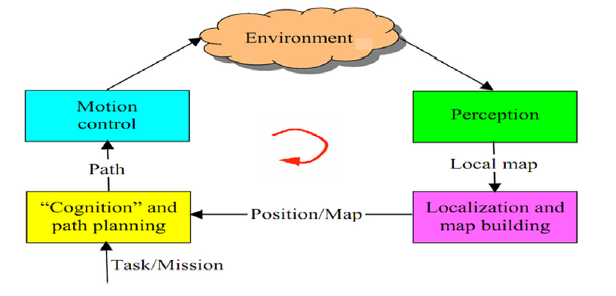
\includegraphics[scale=0.8]{architetturaNavigazione.png}
\label{arch}
\end{figure}

In questa tesi viene affrontato un problema che rientra nel terzo modulo: il path planning, un problema di grande importanza e argomento di molta ricerca.

\subsection{Path planning}

Una sua rapida formulazione potrebbe essere la seguente: data la posizione iniziale (del robot) A e una posizione finale B, imposta da chi fa uso del robot, il path planning consiste nel calcolare un percorso fisicamente realizzabile e ottimale per arrivare da A a B.
All'interno dei metodi esistenti (e non), ci sono due importanti distinzioni da fare: sulla formulazione del problema e sulla soluzione al problema.
\begin{description}
\item[La prima] é tra online e offline path planning, o anche locale e globale. Il path planning globale riguarda quelle situazioni in cui l'ambiente considerato é interamente noto a priori, per cui é possibile calcolare il percorso da seguire ancor prima che il robot inizi a muoversi; quello locale é inerente ai casi in cui il robot debba fare i conti lungo il suo percorso con eventi inaspettati, quali ostacoli dinamici,per cui é necessario reagire localmente, aggiornando ripetutamente le informazioni derivanti dai sensori e aggiustando la traiettoria al fine di evitare l'ostacolo e poter raggiungere in tempi ottimali l'obiettivo. Chiaramente, la maggior parte dei problemi di robotica autonome deve fare i conti con una situazione del secondo tipo. 
\item[La seconda] distinzione é tra soluzioni basate su tecniche di intelligenza artificiale - la cui trattazione esula dagli scopi di questa tesi - e soluzioni classiche. Queste ultime possono ulteriormente essere suddivise in \cite{siciliano}:
\begin{itemize}
\item Subgoal (o anche roadmap), la cui realizzazione più nota é il metodo che sfrutta i diagrammi di Voronoi. 
\item Decomposizione in celle
\item Sampling based che frutta un approccio probabilistico.
\item Potenziali artificiali, che verranno ampiamente in trattati nel prossimo capitolo
\end{itemize}
\end{description}

Di seguito si descriverá brevemente degli esempi legati ai metodi appena elencati.

\paragraph{Voronoi} L'idea alla base di questo metodo é rappresentare lo spazio libero delle configurazioni \(C_{free}\), ovvero l'insieme di quei punti che per certo non fanno collidere il robot con un ostacolo, come un grafo, ovvero un insieme di nodi (rappresentati appunto la roadmap) connessi da archi. La posizione dei nodi é definita tramite il concetto di clearance, ovvero la funzione \[\gamma(q) = \min_{s\in\partial C_{free}} \begin{Vmatrix}q-s\end{Vmatrix}\] dove q é una generica configurazione in \(C_{free}\). \(\partial C_{free}\) sarebbe la frontiera dello spazio di configurazione, ovvero il bordo degli ostacoli. Il grafo é formato da quelle configurazioni \(q\) tali per cui esiste più di un punto su \(\partial C_{free}\) con lo stesso valore \(\gamma(q)\). In altre parole, quei punti equidistanti (considerando la distanza minima) da più di un ostacolo. Il risultato é quello mostrato in figura \ref{voronoi}. Una volta calcolato il grafo, é sufficiente ritrarre i punti di start e goal sul grafo stesso e calcolare il percorso ottimale tra questi due attraverso un algoritmo di ricerca, ad esempio Djikstra.

\paragraph{Decomposizione esatta in celle} In questa tecnica lo spazio delle configurazioni viene suddiviso in celle, come mostrato in figura \ref{celldecomp}. Ogni cella é delimitata inferiormente e superiormente da un ostacolo e ogni cella ha le seguenti due caratteristiche:
\begin{itemize}
\item Tra ogni coppia di configurazioni nella stessa cella esiste sempre un cammino senza collisioni
\item Tra ogni coppia di celle adiacenti esiste sempre un cammino senza collisioni (che conduce da una cella all'altra)
\end{itemize}
In base a questi due principi, viene costruito il cosiddetto grafo di connettività, che ha come archi le connessioni tra celle adiacenti. Come nel metodo precedente, il calcolo del percorso ottimale per raggiungere il goal consiste nell'applicare un algoritmo di ricerca su grafo.

\begin{figure}[h]
\begin{subfigure}[t]{0.5\textwidth}
\centering
\caption{Diagramma di Voronoi}
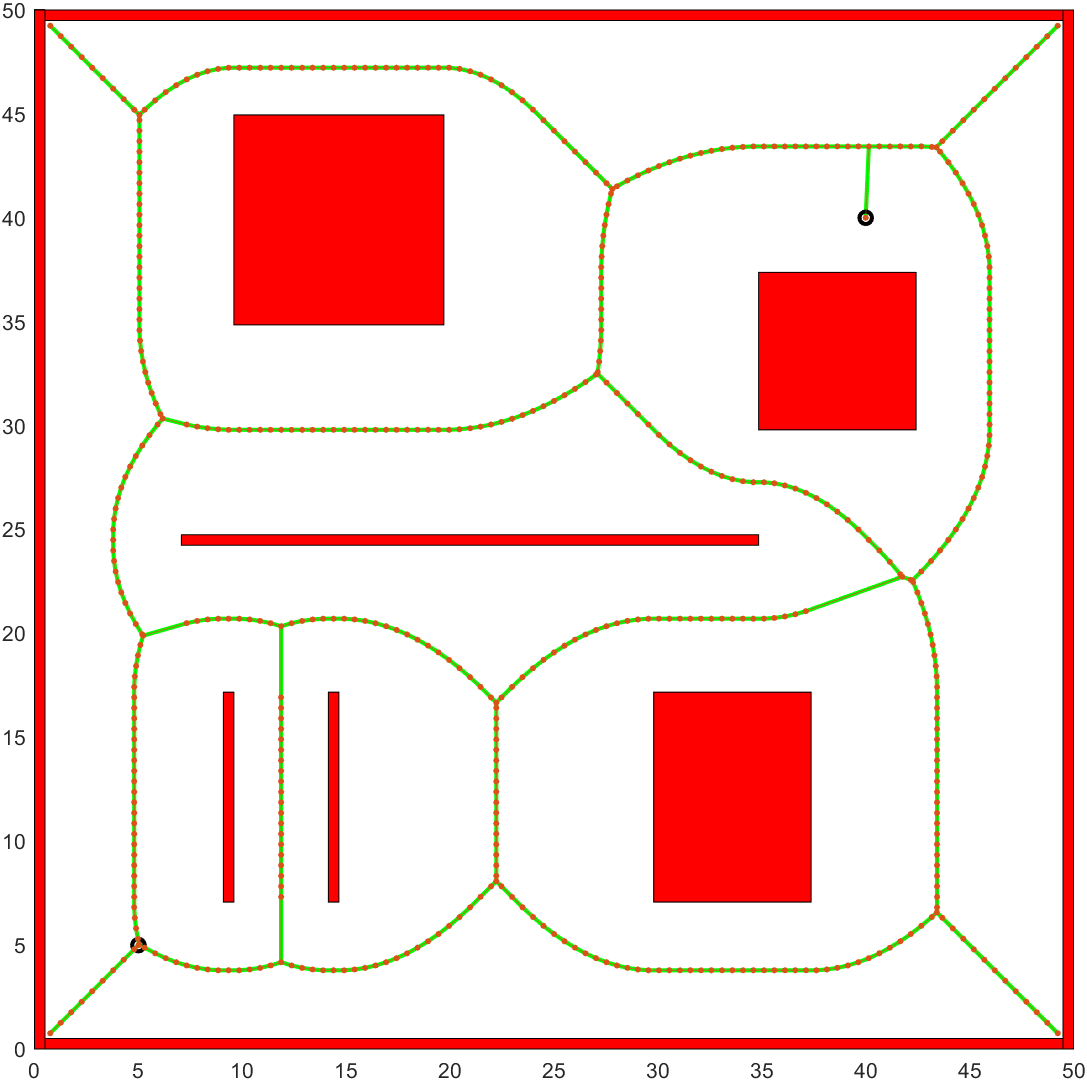
\includegraphics[width=\textwidth]{voronoi.png}
\label{voronoi}
\end{subfigure}
\hfill
\begin{subfigure}[t]{0.5\textwidth}
\centering
\caption{Decomposizione in celle}
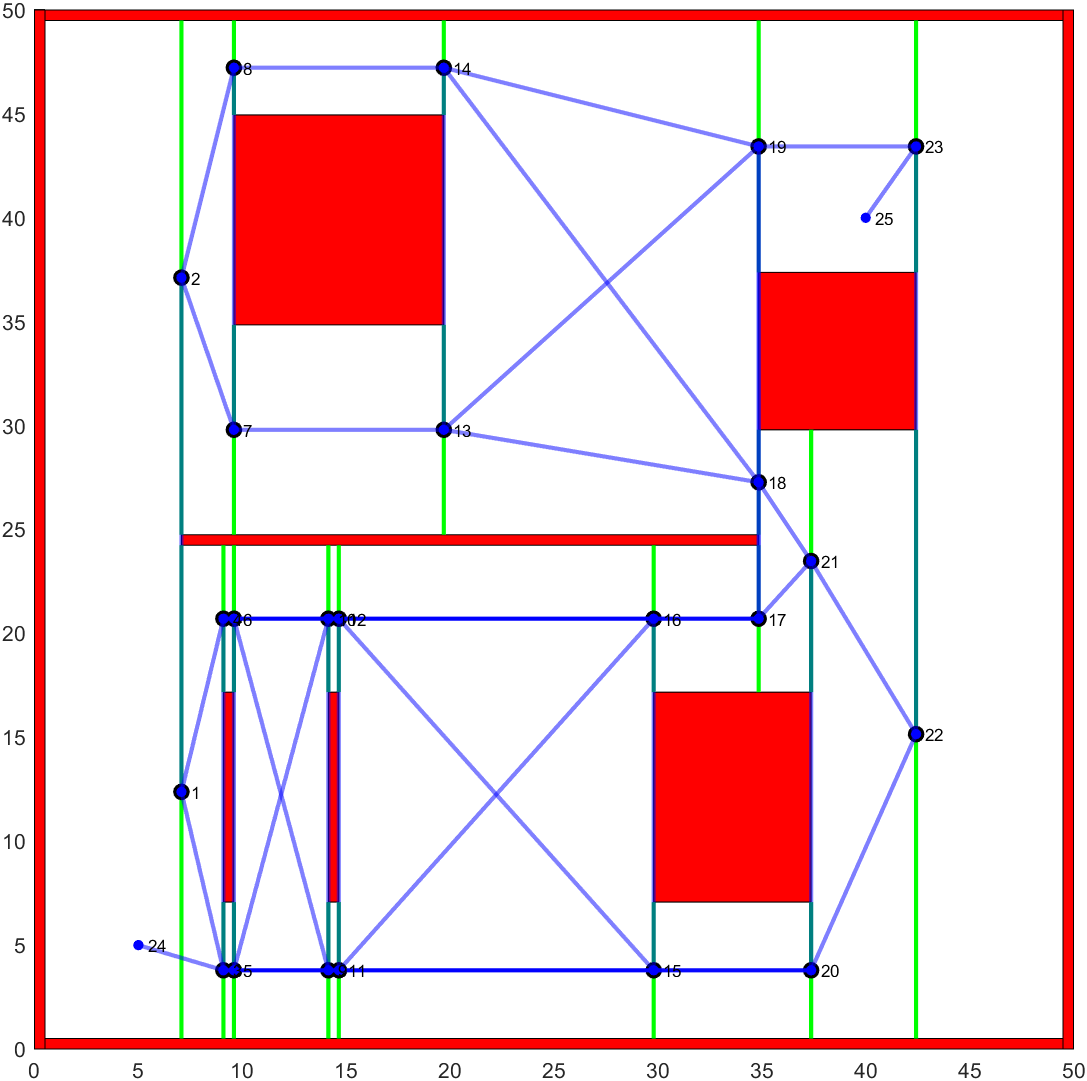
\includegraphics[width=\textwidth]{celldecomp.png}
\label{celldecomp}
\end{subfigure}
\caption{Metodi classici basati su grafo}
\end{figure}

\paragraph{Sampling based} Il terzo metodo si basa su un approccio probabilistico. Brevemente, l'idea é di scegliere a ogni iterazioni una configurazione "di prova" e fare un test di collisione su quest'ultima e si cerca di collegare in basa alla vicinanza alle configurazioni giá appartenenti al grafo che si sta costruendo. \\


La breve descrizione dei metodi serviva anche a motivare la scelta dei potenziali artificiali come base per lo sviluppo dell'algoritmo di navigazione, visto che la totalità dei metodi rientranti nelle prime tre categorie risolve adeguatamente il problema del path planning globale \cite{dalfonso}, ma risulta inefficiente nel caso del path planning locale. Tuttavia, sono particolarmente efficienti nel caso in cui ci si trovi in un ambiente noto a priori, poco incline al cambiamento e con l'esigenza di fare query ripetute. Il costo computazionale é quasi tutto contenuto nel calcolo del grafo, e la singola query ha un costo legato al numero di archi.

\begin{figure}[H]
\caption{Classificazione algoritmi di path planning\cite{mac2016}}
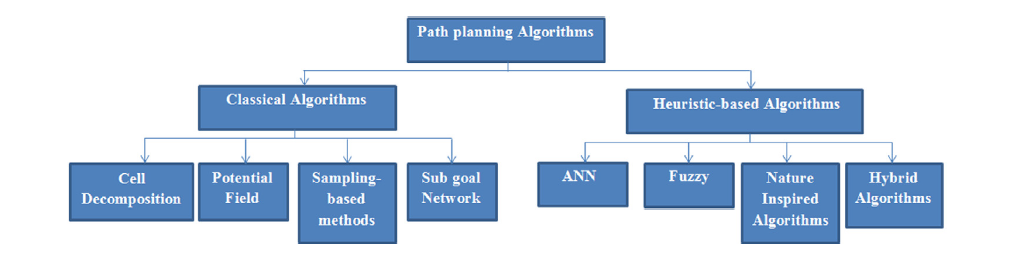
\includegraphics[width=\textwidth]{algoritmiPP.png}
\end{figure}

Come da titolo, questa tesi ha come obiettivo specifico quello di esporre un lavoro di progettazione, implementazione e simulazione di un algoritmo di path planning \textbf{locale} basato su \textbf{potenziali artificiali alternati}. 

\subsection{Formalizzazione del problema}

Chiamerò \( r(t) = [x_r(t),y_r(t),\theta_r(t)]^T\) la posizione del robot nell'istante t e \( O_i(t) = [x_{O,i}(t),y_{O,i}(t)]^T, i = 1...N\) la posizione degli N ostacoli che, per scopi esemplificativi in fase di prototipazione dell'algoritmo, saranno di forma circolare e con raggio \(R_i\). Quest'ultima ipotesi non provoca una perdita di generalità, visto che per un ostacolo di forma generica si può considerare la sua circonferenza circoscritta. Esisterà inoltre un punto \(G = [G_x, G_y]\) che indica l'obiettivo del robot. Il problema consiste nel voler raggiungere il punto \(G\) dalla posizione iniziale \(r(0)\), tenendo conto degli \(N\) ostacoli in movimento. Il robot é dotato di un raggio di visione di \(R_v\) metri, entro il quale é capace di rilevare un ostacolo. Inoltre, si presuppone che valga la seguente condizione
\[\begin{Vmatrix}\begin{bmatrix} x_r(t)\\ y_r(t) \end{bmatrix} - O_j(t)\end{Vmatrix} \leq R_v \], ovvero \( R_i \leq R_v, \forall i\). Ciò vuol dire che nel momento in cui il robot incontra un ostacolo, il centro di quest'ultimo é incluso in \(R_v\). \newpage

\section{Potenziali artificiali}

\subsection{Metodo classico}
Tradizionalmente, nel path planning basato su potenziali artificiali il robot viene fatto muovere mediante una funzione in due variabili, ovvero un potenziale scalare, che nasce dalla somma di due potenziali: attrattivo e repulsivo. Questi due potenziali sono chiamati artificiali perché generano una forza che guida il robot in ogni sua configurazione \( r(t)\), nonostante nella realtà non vi sia nessuna sorgente a generare quella forza. Nello specifico, la forza generata dal potenziale é il suo antigradiente, ovvero il gradiente cambiato di segno, che indica al robot la direzione di moto localmente più promettente\cite{oriolo}, cioè verso il punto di minimo della funzione. Di conseguenza il potenziale attrattivo assume una forma tale da avere un unico punto di minimo posizionato proprio nel punto di arrivo, mentre il repulsivo ha un unico punto di massimo corrispondente alla posizione dell'ostacolo. 

\begin{description}
\item[Il potenziale attrattivo] ha di solito la forma mostrata in figura \ref{potA}, in cui il punto di minimo, ovvero il goal, ha coordinate \([1,1.5]\).
\begin{figure}[H]
\centering
\caption{Potenziale attrattivo}
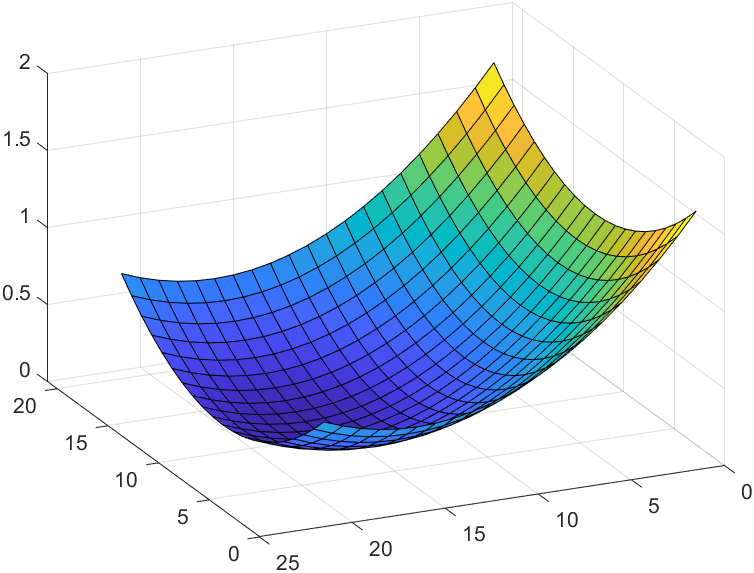
\includegraphics[width=0.8\textwidth]{potA.png}
\label{potA}
\end{figure}

a cui corrisponde la funzione 

\begin{equation}
U_a(r(t),G) = \frac{1}{2} \begin{Vmatrix}G - \begin{bmatrix} x_r(t)\\ y_r(t) \end{bmatrix}\end{Vmatrix}^2
\end{equation}

Il suo antigradiente di conseguenza é formato da tanti vettori che, con un'intensità proporzionale alla distanza dal goal, puntano verso quest'ultimo.
\begin{figure}[H]
\centering
\caption{Antigradiente del potenziale attrattivo}
\label{antigradA}
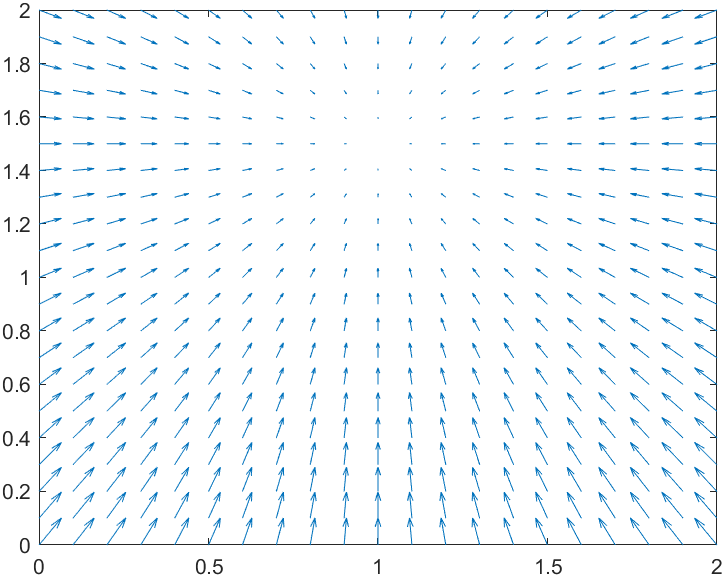
\includegraphics[width=0.6\textwidth]{antigradA.png}
\end{figure} e matematicamente si esprime come il vettore delle derivate parziali (del potenziale) cambiato di segno, ovvero 

\begin{equation}
-\nabla U_a(r(t),G) = \begin{Vmatrix}G - \begin{bmatrix} x_r(t)\\ y_r(t) \end{bmatrix}\end{Vmatrix}
\end{equation}

Perciò, la forza esercitata dal potenziale sul robot punta verso il goal e converge a zero quando la configurazione \(r(t)\) tende alla destinazione \(G\), esprimendo difatti un errore lineare tra goal e posizione del robot. 

\item[Il potenziale repulsivo] ha una forma duale a quello attrattivo, come mostrato in figura \ref{potR}. Esso impone che entro uno distanza \(\eta\) dall'ostacolo per il quale lo si sta calcolando, la sua funzione avrà valore inversamente proporzionale alla distanza dall'ostacolo stesso. Praticamente, più ci si avvicina all'ostacolo entro una certa soglia \(\eta\), più l'intensità del potenziale artificiale, perciò anche della forza generata da esso, aumenta.

\begin{figure}[H]
\begin{subfigure}[t]{0.5\textwidth}
\caption{Potenziale repulsivo}
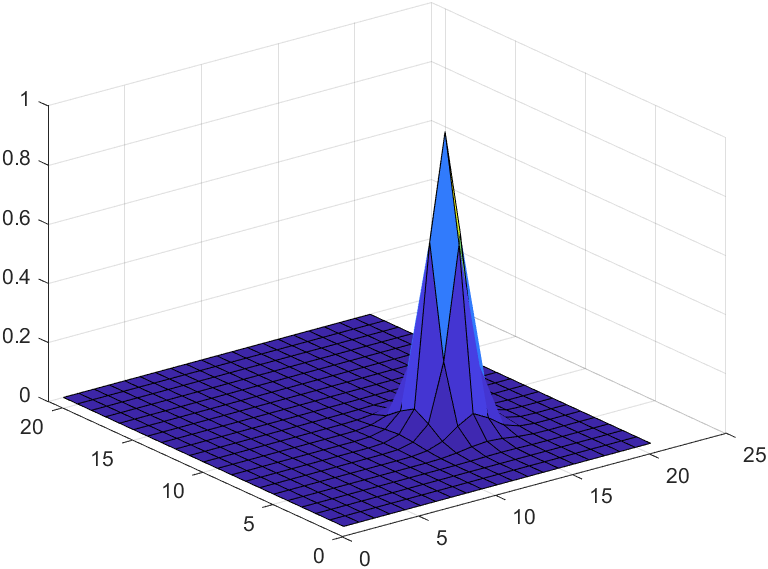
\includegraphics[width=\textwidth]{potR.png}
\label{potR}
\end{subfigure}
\hfill
\begin{subfigure}[t]{0.5\textwidth}
\caption{Antigradiente del potenziale repulsivo}
\label{antigradR}
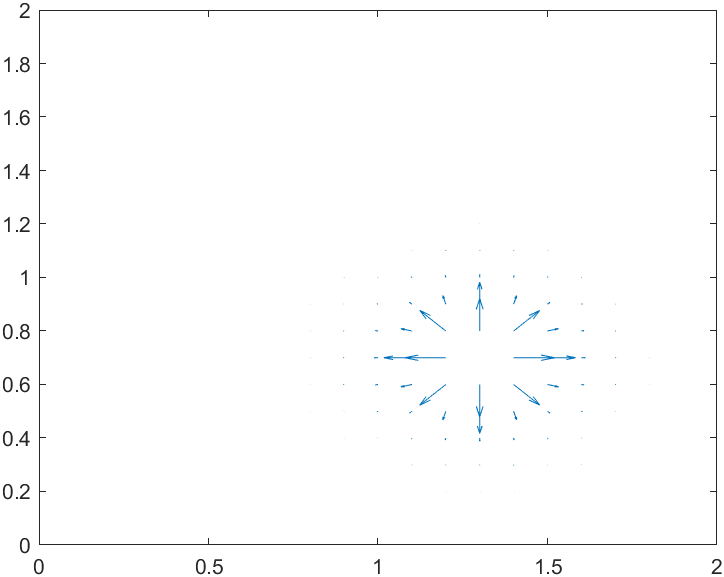
\includegraphics[width=\textwidth]{antigradR.png}
\end{subfigure}
\caption{Potenziale repulsivo}
\end{figure}

Al potenziale repulsivo corrisponde la seguente funzione a tratti 

\begin{equation}
\label{potREq}
U_r(r(t),O_j(t)) = 
\begin{cases}
\frac{1}{2} \left( \frac{1}{d(r(t),O_j(t)} - \frac{1}{\eta} \right) \quad &d(r(t),O_j(t)) \leq \eta \\
0 \quad &altrimenti
\end{cases}
\end{equation}
dove \[ d(r(t),O_j(t) = \begin{Vmatrix}O_j(t) - \begin{bmatrix} x_r(t)\\ y_r(t) \end{bmatrix}\end{Vmatrix}\]

Dunque, il compito della forza generata é quello di spingere via il robot dalla posizione dell'ostacolo tanto più che il robot si avvicina entro la soglia \(\eta\) a quest'ultimo. In figura \ref{antigradR} si vedono le linee di campo dell'antigradiente che puntano radialmente verso l'esterno rispetto alla posizione dell'ostacolo, qui con coordinate \([1.5, 1]\).

\end{description}

Una volta calcolato il potenziale repulsivo per ogni singolo ostacolo (in questo caso uno solo), si ottiene il potenziale totale:

\begin{equation}
U(r(t)) = U_a(r(t),G) + \sum_{j=1}^{n} U_r(r(t),O_j(t))
\end{equation}

In figura \ref{pot} si vede un possibile percorso del robot per arrivare dal punto di partenza al goal. Il vettore velocità del robot \([v_x(t) , v_y(t)]\) ha come riferimento in ogni istante t il valore dell'antigradiente (che é un vettore) in \(r(t)\). Lontano dagli ostacoli, il vettore velocità ha una direzione che punta al goal e un'intensità che diminuisce man mano che ci si avvicina al goal. Più il robot si avvicina ad un ostacolo, più la direzione del vettore velocità vira verso il verso opposto rispetto a \(\theta = \tan \left( \frac{y_{O,j}(t)-y_r(t)}{x_{O,j}(t)-x_r(t)} \right) \) (ovvero la direzione del vettore che collega il robot all'ostacolo), spostando così temporaneamente la traiettoria desiderata e aumentando "l'intensità della virata" lontano dall'ostacolo man mano che si avvicina ad esso.
Il robot dunque, seguendo l'antigradiente, viene in ogni sua configurazione \(r(t)\) - usando l'analogia con il campo gravitazionale - attratto dal goal e \textbf{contemporaneamente} respinto dagli ostacoli. Chiaramente, il metodo é idoneo sia al path planning globale che a quello locale (basta ricalcolare il potenziale totale in presenza di ostacoli). Volendo, però, dare un'etichetta dal punto di vista dell'architettura di navigazione, i potenziali artificiali tradizionali obbediscono ad una di tipo reattivo: considerando la figura \ref{arch}, il modulo di mapping e path planning sono praticamente assenti. Gli attuatori del robot, che sono collegati ai sensori tramite una funzione di trasferimento \cite{kim}, ricevono direttamente il comando derivante dal calcolo del potenziale artificiale, quasi senza alcun tipo di pianificazione algoritmica. 

\begin{figure}[H]
\centering
\caption{Potenziale totale}
\label{pot}
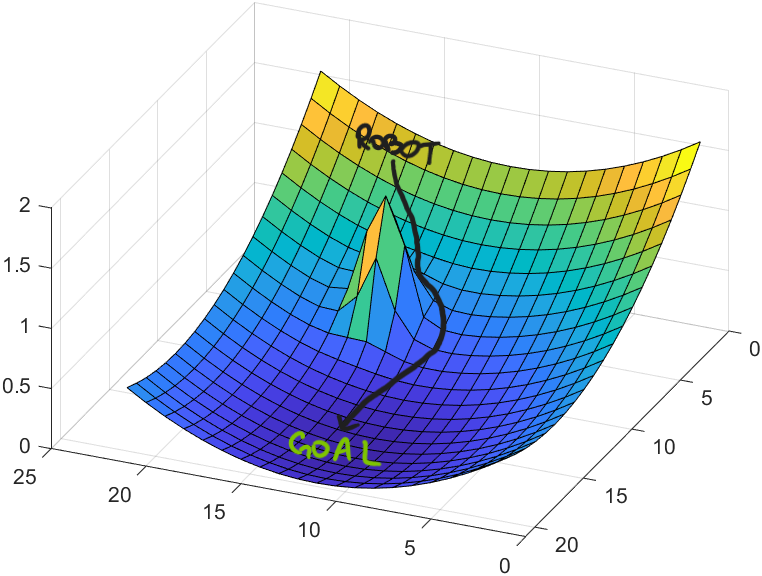
\includegraphics[width=0.7\textwidth]{pot.png}
\end{figure}

Tuttavia, vi sono delle non-idealità legate a questo approccio. Ad esempio, la traiettoria potrebbe non essere continua. Il potenziale repulsivo non é "coordinato" con quello attrattivo, perciò il robot potrebbe ricevere comandi che causerebbero un cambio di direzione o di velocità troppo repentino che andrebbe gestito dalla legge di controllo o un modulo di pianificazione apposito. Questa osservazione verrà trattata nel capitolo riguardante l'algoritmo di navigazione. \\
Altro problema da considerare é il fatto che il robot viene "passivamente" spinto via dagli ostacoli senza la certezza che venga portato in una posa in cui può effettivamente evitare con successo l'ostacolo.\\
Ma il più importante, sicuramente, é il problema dei minimi locali: il robot non ha alcuna informazione su come uscirne, né può prevederli in anticipo. I minimi locali sono dei punti ad antigradiente nullo (i gradiente del potenziale attrattivo e repulsivo possono annullarsi a vicenda), dove il robot non ha nessuna forza a guidarlo verso il goal, situazione che dovrebbe verificarsi soltanto nel punto di goal stesso. In figura \ref{minloc} viene mostrato il percorso simulato di un robot in presenza di un minimo locale nel potenziale artificiale. Il robot parte dalla posizione \(r(0) = [5,0]\) mentre il goal si trova in posizione \(G = [5,10]\). Gli ostacoli sono posizionati tra il robot e il goal ad una distanza tale da causare un annullamento del gradiente (quindi il minimo locale) proprio a metà tra i due, lì dove il robot cerca di passare. La traiettoria del robot, infatti, si ferma nel minimo locale: non viene spinto da nessuna forza e "crede" di essere arrivato nel punto di goal.
\begin{figure}[H]
\begin{subfigure}[t]{0.5\textwidth}
\caption{Potenziale con minimo locale}
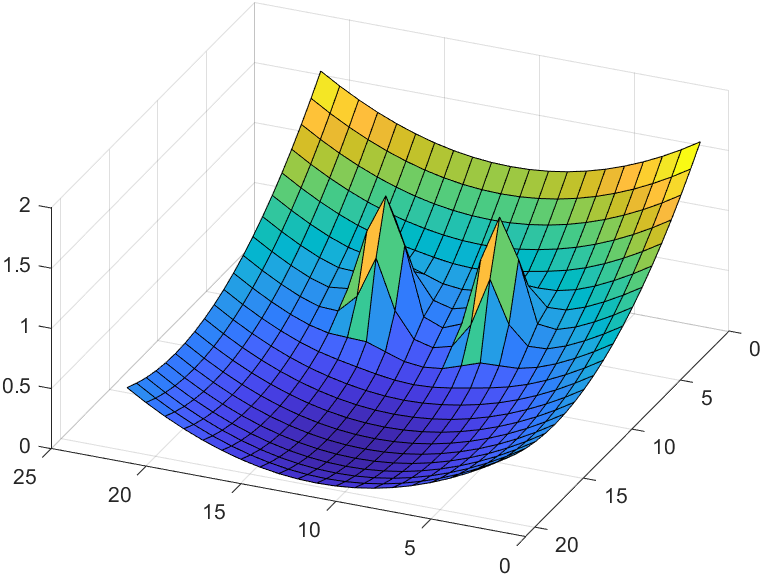
\includegraphics[width=\textwidth]{minimoLocale.png}
\end{subfigure}
\hfill
\begin{subfigure}[t]{0.5\textwidth}
\caption{Antigradiente del potenziale con minimo locale}
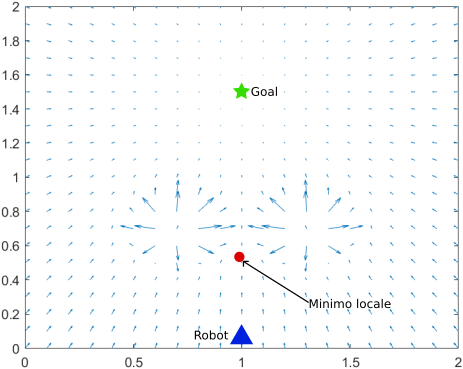
\includegraphics[width=\textwidth]{antigradMinimoLocale.png}
\end{subfigure}
\caption{Minimo locale}
\label{minloc}
\end{figure}

\subsection{Potenziale bypassante}
Al fine di evitare le non-idealità dovute all'utilizzo dei potenziali sommati, l'idea implementata in questa tesi é quella di sfruttare al posto di quello repulsivo un altro tipo di potenziale che chiameremo bypassante. Fondamentalmente, si tratta di un potenziale che invece di spingere via il robot dall'ostacolo, lo porta a circumnavigarlo. Infatti, le linee di campo dell'antigradiente di questo potenziale sono concentriche, al contrario di quelle del potenziale repulsivo che sono radiali. L'idea quindi é di basarsi su una superficie che ruoti attorno a un centro, identificato dalla posizione, ad esempio un elicoide:

\begin{equation}
\begin{cases}
x = x_0 + r cos(\xi) \\
y = y_0 + r sin(\xi)  \\
z = c \xi
\end{cases}
\end{equation}

Applicando nella terza equazione la tangente da entrambe le parti, otteniamo \(\tan(\xi)=\tan(\frac{z}{c})\) che, confrontando con le prime due equazioni, diventa
\[\tan \left( \frac{z}{c} \right) = \frac{y-y_0}{x-x_0}\] dove \([x_0,y_0]\) sarebbe la posizione dell'ostacolo. Invertendo questa funzione per esprimerla come z in funzione di x e y, otteniamo il potenziale elicoidale, ridenominato bypassante, in senso orario rispetto all'ostacolo e centrato in esso:

\begin{equation}
\label{potBeq}
\Gamma(x,y,x_0,y_0) = c\tan^{-1} \left( \frac{y-y_0}{x-x_0} \right)
\end{equation}

\begin{figure}[H]
\begin{subfigure}[t]{0.5\textwidth}
\caption{Elicoide centrato in \([1,1]\) \\ con \(c=2\), \(0\leq r \leq 1\) e \(0 \leq \xi \leq 4\pi\)}
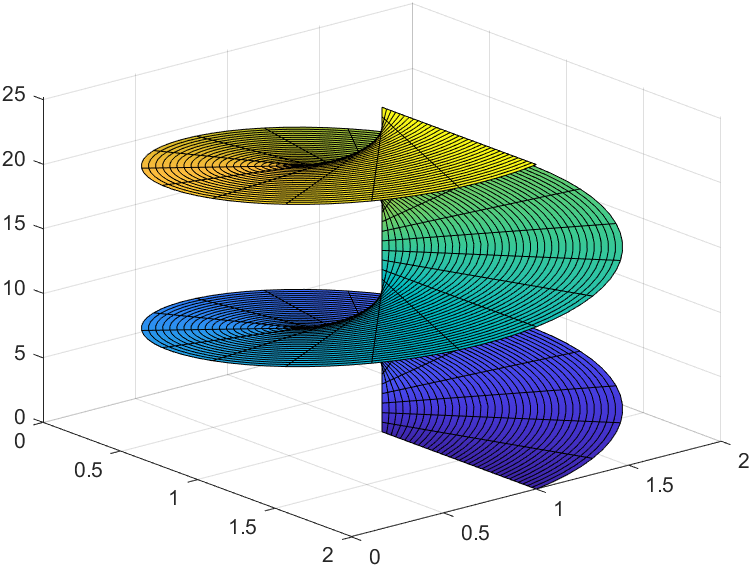
\includegraphics[width=\textwidth]{elicoide.png}
\end{subfigure}
\hfill
\begin{subfigure}[t]{0.5\textwidth}
\caption{Potenziale bypassante centrato in \([1,1]\) con \(c=2\) e in senso orario}
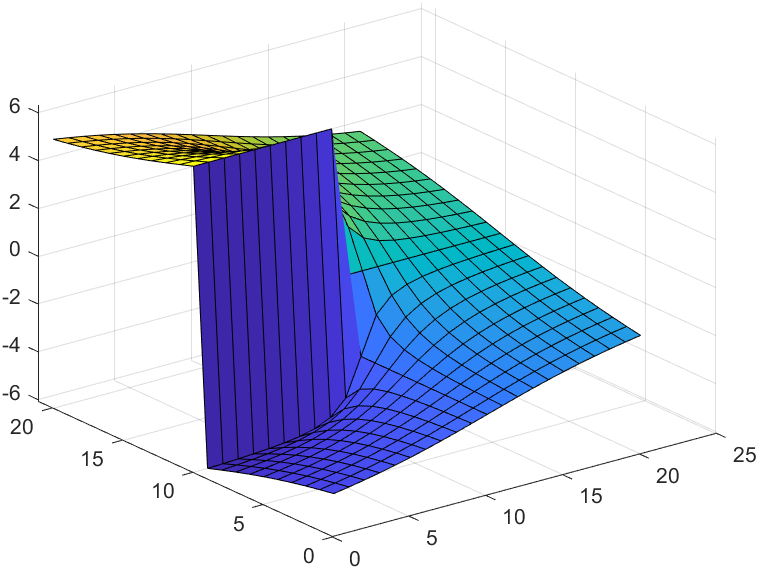
\includegraphics[width=\textwidth]{potB.png}
\label{potB}
\end{subfigure}
\caption{Potenziale bypassante}
\end{figure}

Da notare che il potenziale in figura \ref{potB} ha una discontinuità per \(x=x_0\), per cui la funzione é continua per \((x,y) neq (x_0,y_0)\). Siccome il robot non può mai andare esattamente nella stessa posizione dell'ostacolo, non c'è perdita di generalità nell'ignorare la discontinuità e di conseguenza il robot sarà sempre in grado di seguire la forza generata dal potenziale. Il potenziale con equazione \ref{potBeq} può essere visto come una funzione della posizione del robot e dell'ostacolo da aggirare \[\Gamma(x,y,x_0,y_0) = \Gamma(x_r(t),y_r(t),x_{O,j}(t),y_{O,j}(t))\] Dunque, la forza generata dal potenziale bypassante é esprimibile come il suo antigradiente

\begin{equation}
-\nabla U_b(r(t),O_j(t)) =
\begin{bmatrix}
\frac{c(y_r(t)-y_{O,j}(t))}{(x_r(t)-x_{O,j}(t))^2 + (y_r(t)-y_{O,j}(t))^2} \\\\
\frac{c(x_{O,j}(t) - x_r(t))}{(x_r(t)-x_{O,j}(t))^2 + (y_r(t)-y_{O,j}(t))^2}
\end{bmatrix}
\end{equation}\\

Quindi, l'antigradiente é formato da tanti vettori che
\begin{itemize}
\item Indicano una velocità desiderata nella posa \(r(t)\) del robot, al fine di aggirare l'ostacolo preso in considerazione  \item Aumentano di intensità man mano che il robot si avvicina all'ostacolo
\item Hanno forma concentrica
\end{itemize}

\begin{figure}[H]
\centering
\caption{Antigradiente del potenziale bypassante}
\label{antigradB}
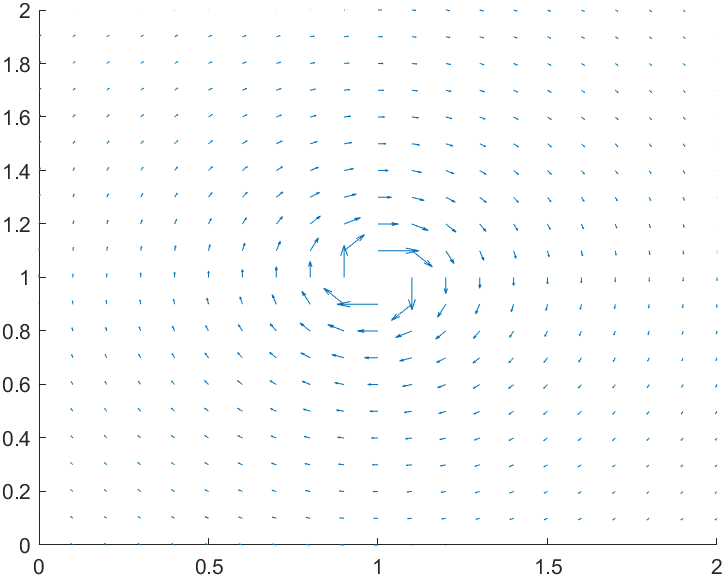
\includegraphics[width=0.8\textwidth]{antigradB.png}
\end{figure}

Questo tipo di potenziale, chiaramente, é intrinsecamente adatto adatto ad ostacoli di forma circolare, motivo per cui nel lavoro di tesi si é considerato soltanto questo tipo di ostacoli.

\section{Algoritmo di navigazione\cite{dalfonso}} 
La strategia é semplice: nella posizione iniziale, il robot sonda l'ambiente attorno a sé. Se non vi sono presenti ostacoli a impedirne l'avanzamento verso il goal, la traiettoria da seguire é quella imposta dal potenziale attrattivo; altrimenti, é necessario "switchare" dal potenziale attrattivo a quello vorticoso, al fine di aggirare l'ostacolo, per poi tornare a seguire la traiettoria. Perciò, la peculiarità di questo algoritmo é che in ogni istante il robot seguirà un solo potenziale alla volta, evitando così il problema dei minimi locali. Inoltre, le informazioni necessarie a pianificare lo switch non richiedono informazioni globali, ma solo relative all'ostacolo da aggirare.

\subsection{Interazione con l'ambiente}
Come viene costruito l'ambiente (grid)\\
\subsubsection{Percezione}
Come vengono percepiti gli ostacoli e le loro velocità\\
Come viene percepita la propria posizione (accenno localizzazione)\\
\subsubsection{Azione}
Modello cinematico\\
Legge di controllo\\
Come faccio muovere il robot nella grid

\subsection{Pianificazione}
Data la struttura intrinseca della strategia di navigazione che si basa su un meccanismo di switching tra due stati, per definizione mutuamente esclusivi, un modo per modellare visivamente l'algoritmo é lo statechart diagram in figura \ref{state}. Il robot può trovarsi o nello stato corrispondente al potenziale attrattivo, oppure in quello corrispondente al potenziale bypassante. In quest'ultimo esistono altri due sottostati, la cui natura verrà spiegata meglio in seguito.
	
\begin{figure}[H]
\caption{Statechart Diagram} \label{state}
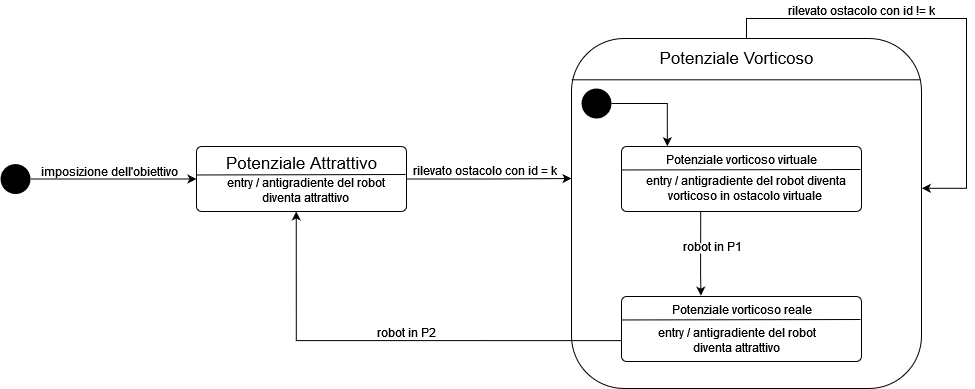
\includegraphics[width=\textwidth]{stateDiagram.png}
\end{figure}
	
Note	: caso 1 sto seguendo il potenziale attrattivo e passo al vorticoso (calcolo verso, calcolo xOmega e yOmega, calcolo P1 e P2, calcolo due potenziali con relativi c), caso 2 sto seguendo il vorticoso e passo all'attrattivo (reimposto attrattivo)
	
\begin{figure}[H]
\caption{Flowchart Diagram} \label{flow}
\centering
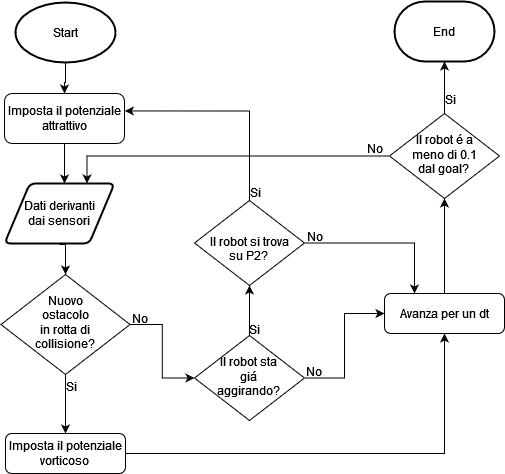
\includegraphics[width=0.8\textwidth]{flowchartDiagram.png}
\end{figure}

\section{Simulazione sul Turtlebot}

\section{Testing e risultati}
Parametri utilizzati\\
Un ostacolo fermo e in movimento\\
Minimi locali e confronto con potenziali artificiali classici\\
Tre in movimento\\

\section{Applicazioni e sviluppi futuri}

\newpage
\listoffigures
\printbibliography

\end{document}